\documentclass[12pt,twoside]{article}

\newcommand{\reporttitle}{CO496 - Mathematics for Inference and Machine Learning}
\newcommand{\reportauthor}{Daren Sin}
\newcommand{\reporttype}{Coursework}
\newcommand{\cid}{ds2912}

% include files that load packages and define macros
\input{includes} % various packages needed for maths etc.
\input{notation} % short-hand notation and macros


%%%%%%%%%%%%%%%%%%%%%%%%%%%%

\begin{document}
% front page
\input{titlepage}

\section*{Part I}

The plots for the YALE and PIE datasets can be found in Figure \ref{fig:part1YALE} and \ref{fig:part1PIE} respectively.

First, for both datasets, LDA and PCA with whitening performed significantly better, with much lower test errors compared to the default PCA, across all dimensions. 

\begin{figure}
  \centering
    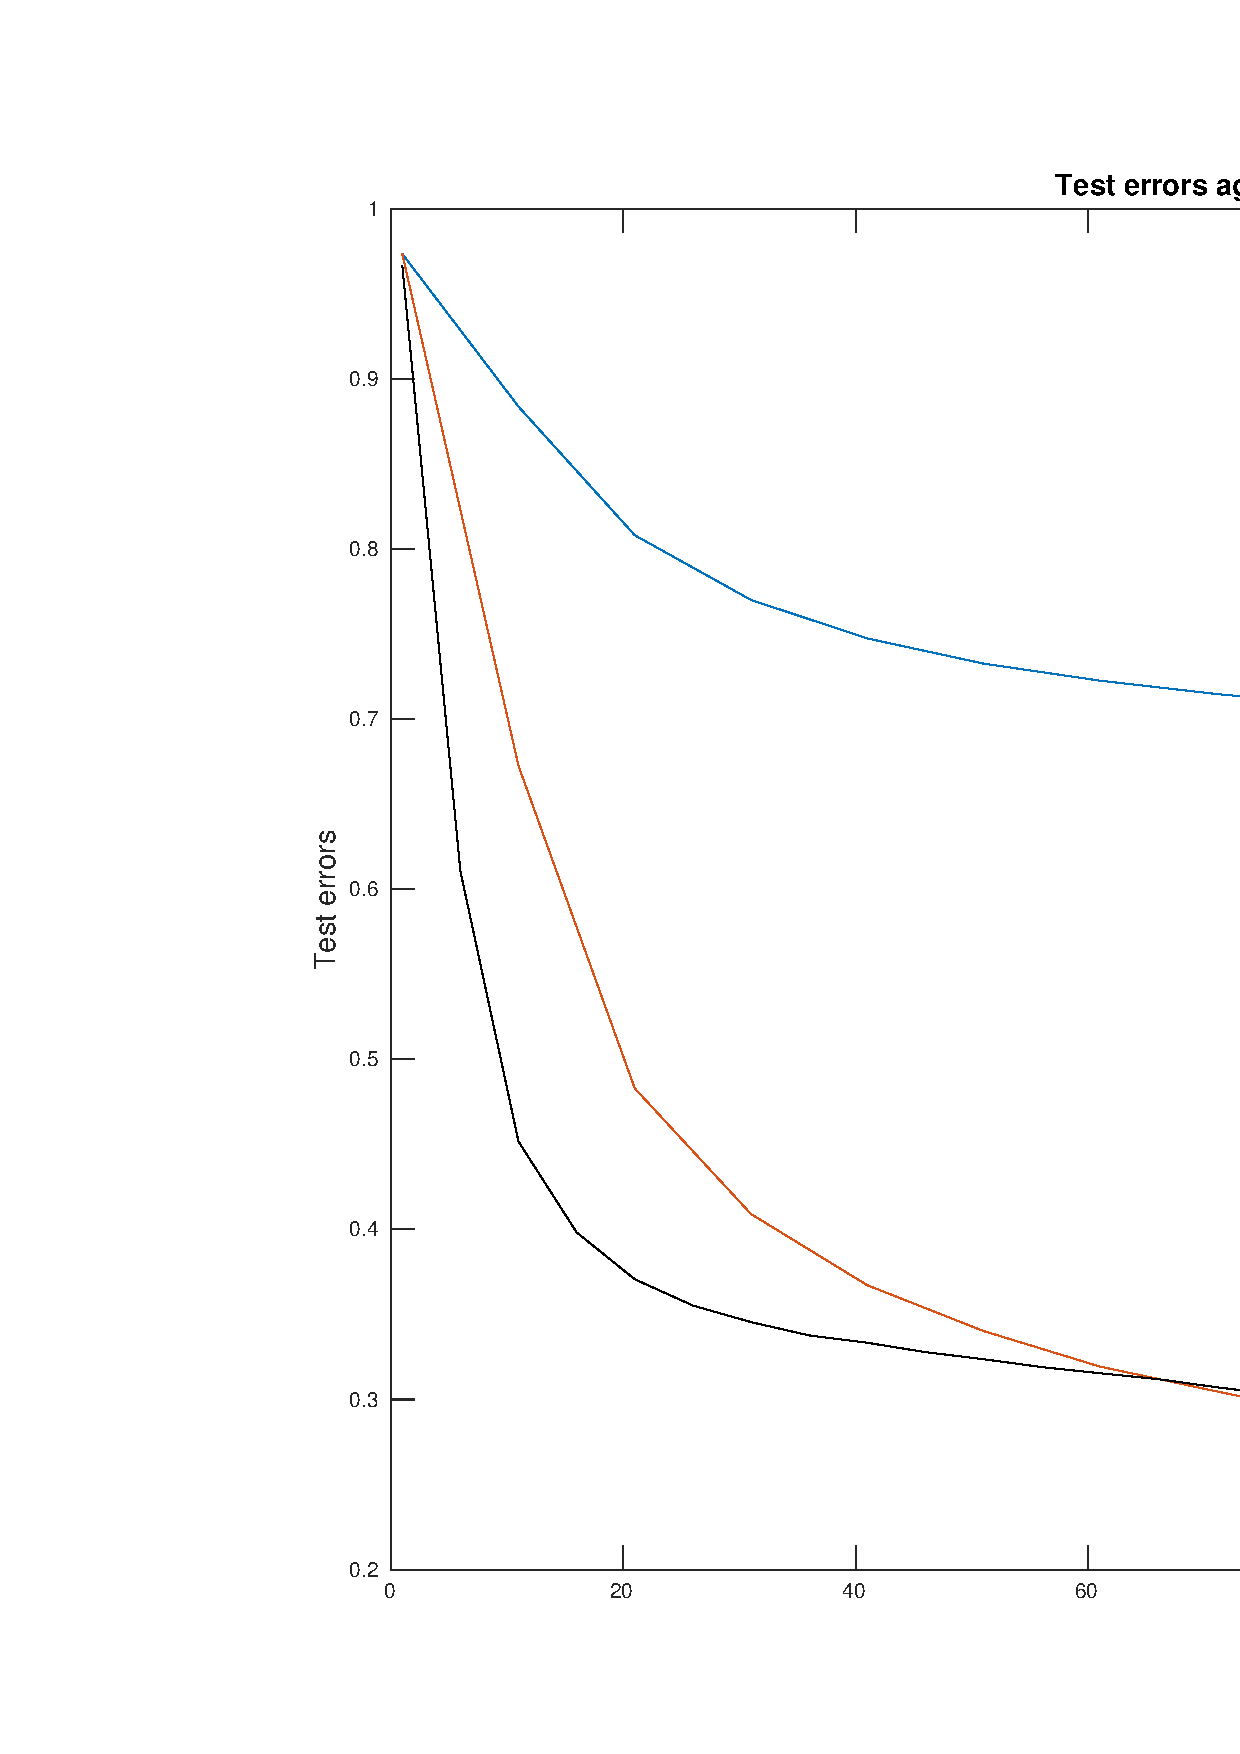
\includegraphics[scale = 0.26]{./figures/YALE.jpg}
  \caption{Graph of test errors against number of dimensions for the YALE dataset.}
  \label{fig:part1YALE}
\end{figure}

\begin{figure}
  \centering
    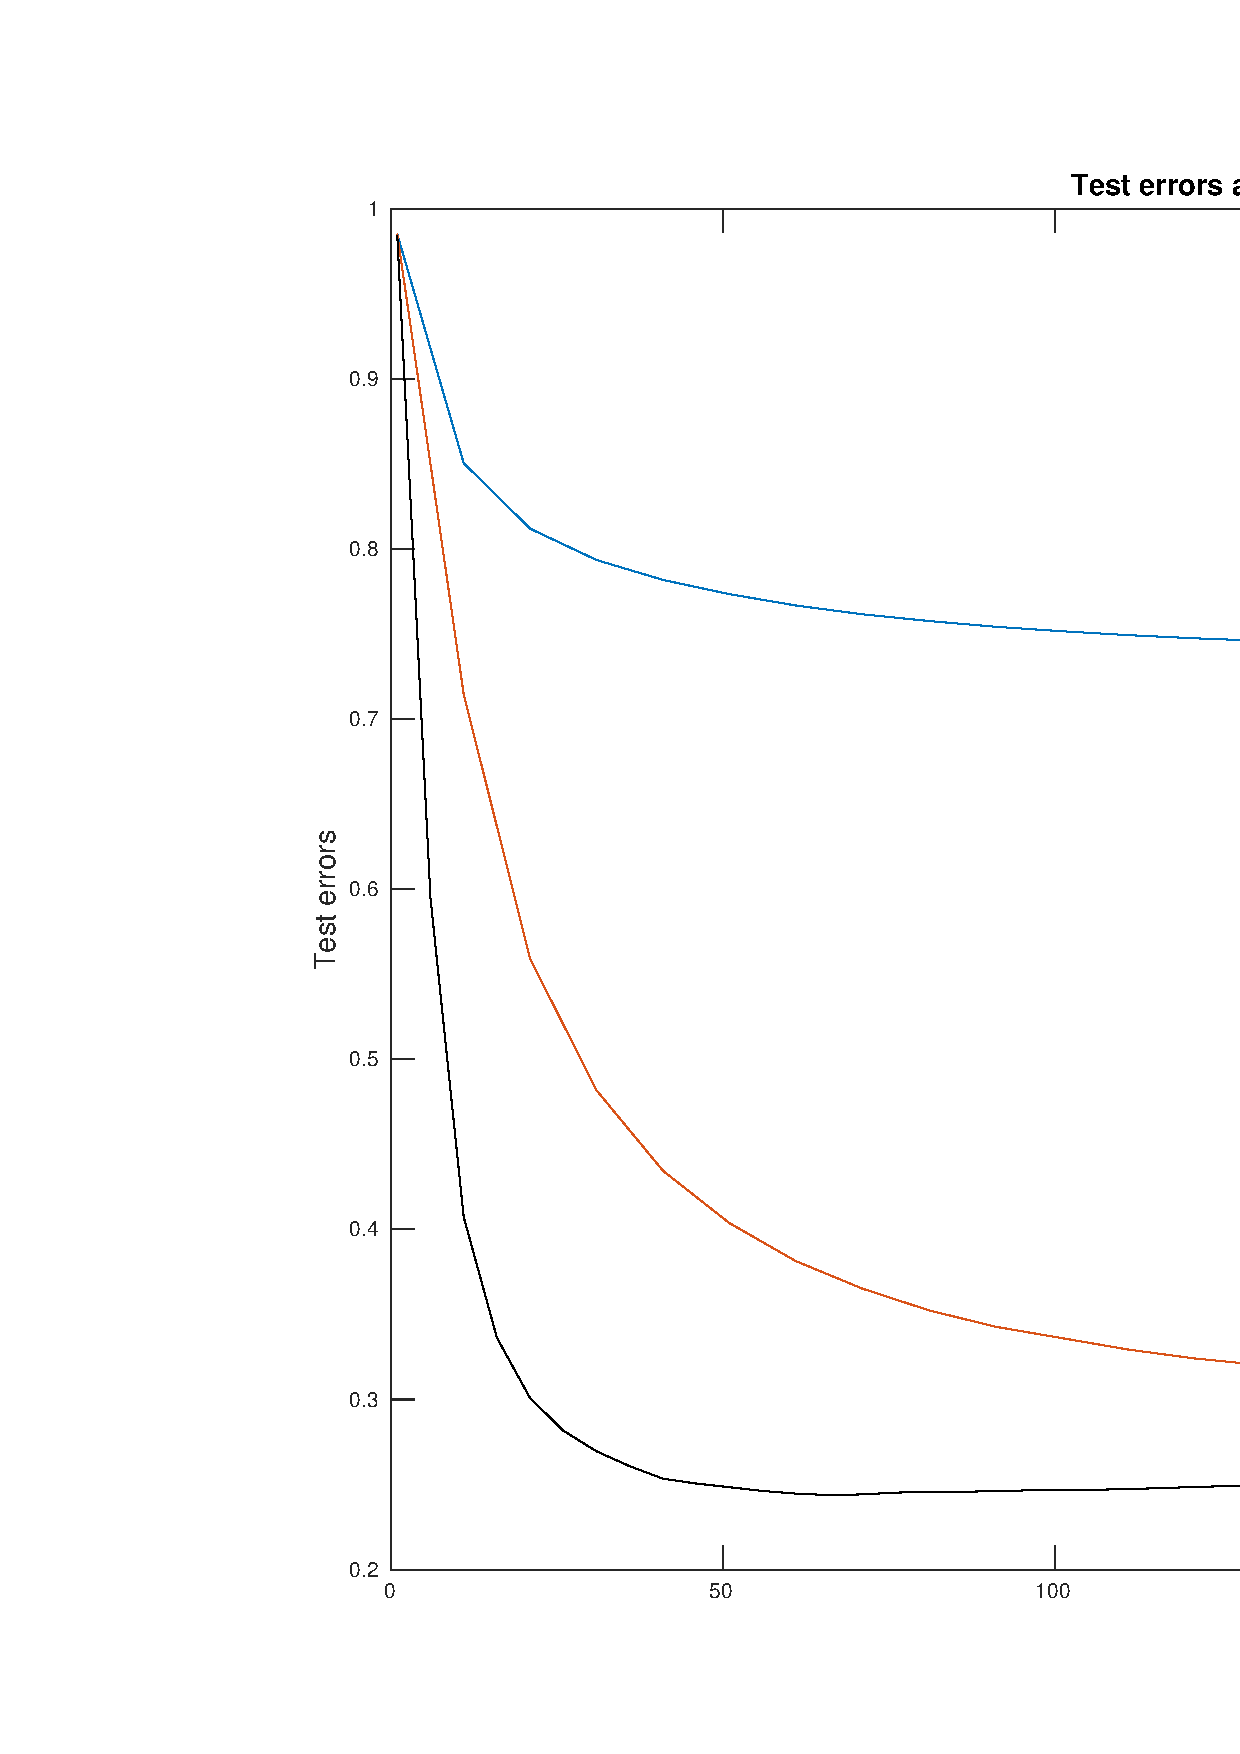
\includegraphics[scale = 0.26]{./figures/PIE.jpg}
  \caption{Graph of test errors against number of dimensions for the PIE dataset.}
  \label{fig:part1PIE}
\end{figure}

\section*{Part II}

\begin{enumerate}[1.)]
\item

The Lagrangian is as follows:
\begin{align}
L(R, \vec a, \xi_i, \lambda, r)
&= R^2 + C \sum_{i=1}^n \xi_i + \sum_{i=1}^n \lambda_i \left[ (\vec x_i - \vec a)\T (\vec x_i-\vec a) - R^2 - \xi_i \right] - \sum_{i=1}^n r_i \xi_i
\end{align}

To find the dual, we need to minimise the Lagrangian with respect to $R$, $\vec a$, and $\xi_i$. We thus differentiate the Lagrangian with respect to these variables:
\begin{align}
\frac{\partial L}{\partial R} &= 2R - 2R \sum_{i=1}^n \lambda_i \overset{!}{=} 0 \quad \Rightarrow \quad 1 - \sum_{i=1}^n \lambda_i = 0 \quad \Rightarrow \quad \sum_{i=1}^n \lambda_i = 1 \label{partTwodldr} \\
\frac{\partial L}{\partial \vec a} &= \sum_{i=1}^n \lambda_i \left[ -2(\vec x_i - \vec a) \right] \overset{!}{=} 0 \quad \Rightarrow \quad \sum_{i=1}^n \lambda_i(\vec x_i - \vec a) = 0 \label{partTwodlda} \\
\frac{\partial L}{\partial \xi_i} &= C - \lambda_i - r_i \overset{!}{=} 0 \quad \Rightarrow \quad C = \lambda_i + r_i \label{partTwodldxi}
\end{align}

Furthermore, from equation \ref{partTwodlda}, we also have the result:
\begin{align}
\sum_{i=1}^n (\lambda_i \vec x_i - \vec a \lambda_i) = 0 \quad \Rightarrow \quad \sum_{i=1}^n (\lambda_i \vec x_i) - \vec a = 0 \quad \Rightarrow \quad \vec a = \sum_{i=1}^n \lambda_i \vec x_i \label{partTwoResultA}
\end{align}
using the result that $\sum_{i=1}^n \lambda_i = 1$ from above. So, using the above equations, we can express the Lagrangian as such:
\begin{align}
L(\lambda)
&= R^2 + \sum_{i=1}^n (\lambda_i + r_i) \xi_i + \lambda_i \sum_{i=1}^n (\vec x_i - \vec a)\T (\vec x_i - \vec a) - R^2 \sum_{i=1}^n \lambda_i - \sum_{i=1}^n \lambda_i \xi_i - \sum_{i=1}^n r_i \xi_i \\
&= R^2 + \sum_{i=1}^n (\lambda_i + r_i) \xi_i + \sum_{i=1}^n \left[ \lambda_i \, (\vec x_i - \vec a)\T (\vec x_i - \vec a) \right] - R^2 - \sum_{i=1}^n (\lambda_i + r_i) \xi_i \\
&= \sum_{i=1}^n \left[ \lambda_i \, (\vec x_i\T - \vec a\T) (\vec x_i - \vec a) \right] \\
&= \sum_{i=1}^n \lambda_i \, \left[ \vec x_i\T \vec x_i - \vec x_i\T \vec a - \vec a\T \vec x_i + \vec a\T \vec a  \right] \\
&= \sum_{i=1}^n \left[ \lambda_i \vec x_i\T \vec x_i - \lambda_i \vec x_i\T \vec a - \lambda_i \vec a\T \vec x_i + \lambda_i \vec a\T \vec a \right] \\
&= \sum_{i=1}^n \left[ \lambda_i \vec x_i\T \vec x_i - \lambda_i \vec x_i\T \vec a - \lambda_i \vec a\T (\vec x_i - \vec a) \right] \\
&= \sum_{i=1}^n \left[ \lambda_i \vec x_i\T \vec x_i - \lambda_i \vec x_i\T \vec a \right] - \vec a\T \underbrace{\sum_{i=1}^n \lambda_i (\vec x_i - \vec a)}_{=0 \text{, from equation \ref{partTwodlda}}}
\end{align}

We also note that, from equation \ref{partTwoResultA}, we have
\begin{align*}
\vec a = \sum_{j=1}^n \lambda_j \vec x_j
\end{align*}

So,
\begin{align}
L(\lambda)
&= \sum_{i=1}^n \left[ \lambda_i \vec x_i\T \vec x_i - \lambda_i \vec x_i\T \vec a \right] \\
&= \sum_{i=1}^n (\lambda_i \vec x_i\T \vec x_i) - \sum_{i=1}^n \lambda_i \vec x_i \T \left( \sum_{j=1}^n \lambda_j \vec x_j \right) \\
&= \sum_{i=1}^n (\lambda_i \vec x_i\T \vec x_i) -  \sum_{i=1}^n \sum_{j=1}^n \lambda_i \vec x_i \T \vec x_j \lambda_j \\
&= \diag (\mat X\T \mat X)\T \lambda - \lambda\T (\mat X\T \mat X) \lambda \\
&= \diag (\mat K_x)\T \vec \lambda - \vec \lambda\T (\mat K_x) \vec \lambda
\end{align}
where $\mat K_x = [\vec x_i\T \vec x_j]$. Hence, we can write the dual as:
\begin{align*}
\max_\vec\lambda \quad &\diag (\mat K_x)\T \vec \lambda - \vec \lambda\T (\mat K_x) \vec \lambda \\
\text{subject to} \quad &\lambda_i \geq 0, \quad 0 \leq \lambda_i \leq C, \quad \text{for } i = 1, \dots , n \\
&\sum_{i=1}^n \lambda_i = 1 \quad \Rightarrow \quad \vec 1\T \vec \lambda = 1
\end{align*}

The second constraint, $0 \leq \lambda_i \leq C$, for $i = 1, \dots , n$ can be derived from equation \ref{partTwodldxi}, which implies that $\lambda_i = C - r_i$. Since $r_i \geq 0$ and $\lambda_i \geq 0$, $r_i$ can only take values from 0 to $C$, inclusive. We then have the constraint, $0 \leq \lambda_i \leq C$.

Furthermore, we can write the above optimisation problem as its equivalent minimisation problem:
\begin{align*}
-\min_\vec\lambda \quad &-\diag (\mat K_x)\T \vec \lambda + \vec \lambda\T (\mat K_x) \vec \lambda \\
\text{subject to} \quad &0 \leq \lambda_i \leq C, \quad \text{for } i = 1, \dots , n \\
&\vec 1\T \vec \lambda = 1
\end{align*}

\item

When using arbitrary positive definite kernels, we can write the above optimisation problem as the following:
\begin{align*}
-\min_\vec\lambda \quad &-\diag (\mat K_x)\T \vec \lambda + \vec \lambda\T (\mat K_x) \vec \lambda \\
\text{subject to} \quad &0 \leq \lambda_i \leq C, \quad \text{for } i = 1, \dots , n \\
&\vec 1\T \vec \lambda = 1
\end{align*}
where $\mat K_x = [k(\vec x_i, \vec x_j)]$ and $k(\vec x_i, \vec x_j) = \phi(\vec x_i)\T \phi (\vec x_j)$ is the kernel.

\item

After identifying the parameters to the MATLAB function \texttt{quadprog} (see MATLAB code), we get an optimal $\vec \lambda^*$ per class, output by the function. We can then substitute the $\vec \lambda^*$ back into the objective function for the dual, to get, say, $-d^*$:

\begin{align*}
-d^* = -\diag (\mat K_x)\T \vec \lambda^* + \vec (\lambda^*) \T (\mat K_x) \vec \lambda^*
\end{align*}

Furthermore, the optimal solution to the primal, $p^*$, is equal to the optimal solution to the dual, $-d^*$, where the negative sign arises from converting our maximisation problem to a minimisation one. We also note that, at the optimal solution, the slack variables, $\xi_i$, go to 0. Hence, keeping $\vec a$ constant, $p^*$ represents the optimal solution to the minimisation problem:
\begin{align*}
R^2 + C \sum_{i=1}^n \xi_i
\end{align*}

As $\xi_i=0$ for all $i = 1, \dots , n$, the optimal $p^*$ is simply the optimal $R^2$. We can thus find the radius of the optimal enclosing hypersphere by taking the square root of $-d^*$. 

We can also find the vector $\vec a_k \in \mathbb{R}^2$, which represents the center of the optimal enclosing hypersphere of class $k$ by:
\begin{align*}
\vec a_k = \sum_{j=1}^n \lambda_j^* \, \vec x_{j,k}
\end{align*}
where $\vec x_{j, k} \in \mathbb{R}^2$ is the $j$th data point of class $k$. The plot of the optimal hyperspheres is in Figure \ref{fig:part2Spheres}.

\begin{figure}
  \centering
    \includegraphics[scale = 0.28]{./figures/sphere.jpg}
  \caption{Plot of data points and the optimal enclosing hyperspheres for each class.}
  \label{fig:part2Spheres}
\end{figure}

\end{enumerate}


\end{document}
